\chapter{Zukünftige Arbeit}
\label{futurework}

Einige bereits angesprochene Punkte bieten Möglichkeiten für eine Erweiterung der hier geleisteten Arbeit.
Während hier ein erheblicher Beitrag zur theoretischen Testabdeckung von GraphQL-APIs geleistet wurde,
so ist nicht garantiert, dass die entwickelten Tests tatsächlich die ermittelte Abdeckung erreichen.
Dies folgert sich aus der zufälligen Argumentgenerierung in den einzelnen Querys.
Ziel ist es nun, den Zufall möglichst weit zu begrenzen oder aber die erlangten Ergebnisse sinnvoller zu nutzen.
Im Folgenden werden zwei Ansätze vorgestellt, die das Potenzial haben, eine praktische Testausführung zuverlässiger und präziser machen zu können.
Ziel von weiterführenden Arbeiten sollte es sein, dass die tatsächliche Pfadabdeckung sich der theoretischen Pfadabdeckung annähert.

\section{BlackBox-Testing in WhiteBox-Testing umwandeln}

Das Testsystem hat im BlackBox-Testing keinerlei Informationen über das SUT und Testgenerierung auf GraphQL-APIs ohne die Argumentgeneratoren anzupassen,
führt häufig dazu, dass die generierten Daten nicht zum SUT passen.
Im experimentellen Ansatz wurde der BlackBox Ansatz abgeschwächt und zu einem GreyBox-Ansatz verändert, indem die Argumentgeneratoren mit Domänenwissen an das jeweilige SUT angepasst wurden,
sodass die zufällige Argumentgenerierung mit höherer Wahrscheinlichkeit ein Argument liefert, das dem Test eine bessere, tatsächliche Abdeckung liefert.
Ideal wäre nun, dass die Testgenerierung auf einem WhiteBox-Ansatz basiert.
Hierdurch ist spezifisches Domänenwissen über das SUT vorhanden, insbesondere dadurch, dass die zugrundeliegenden Daten, Datenstruktur, Programmcode analysierbar sind.
Durch einen White-Box Ansatz wäre es möglich, die Argumentgeneratoren automatisiert anzupassen, sodass sich diese am Schema und den zugrunde-liegenden Daten orientieren.
Außerdem wäre eine Code-Analyse möglich, die dazu führen kann, dass Testfälle noch präziser und exakter Fehler finden.
Die vom Prototypen generierten Testpfade können hierbei weiterhin als Basis dienen, um eine gute Abdeckung sicherzustellen.
Mit optimierten Argumentgeneratoren sollte es möglich sein, die tatsächliche Pfadabdeckung stark zu erhöhen.

\section{Adaptive Generierung}

Die aktuelle Testgenerierung geschieht in einzelnen Phasen.
Es werden erst aus einem Graphen die Pfade generiert, hieraus werden Tests erzeugt und diese werden dann an das SUT gestellt und ausgewertet.
Dabei werden sämtliche Argumente sofort generiert.
Eine adaptive Testgenerierung wäre denkbar, sodass aus einem Testpfad die Query nur in Teilen erstellt wird.
Dabei wird ein Testpfad erst weiter in der Query abgedeckt, wenn ein Argumentgenerator ein Ergebnis zurückliefert, dass die Pfadlänge tatsächlich erhöht und somit signalisiert, dass der zugrundeliegende Test tatsächlich ausgeführt wird.
Eine solche Methode könnte nach dem Ablauf, wie in Abbildung~\ref{adaptive} dargestellt, funktionieren.
Es werden dabei Querys mit Zufallsargumenten erstellt, die einen Teilpfad des Testpfads bilden und erst wenn der Teilpfad des Testpfads tatsächlich abgedeckt ist, wird mit dem nächsten adjazenten Knoten fortgefahren,
sodass die tatsächliche Pfadabdeckung mit der theoretischen Pfadabdeckung übereinstimmt.

\begin{figure}[H]
    \begin{center}
        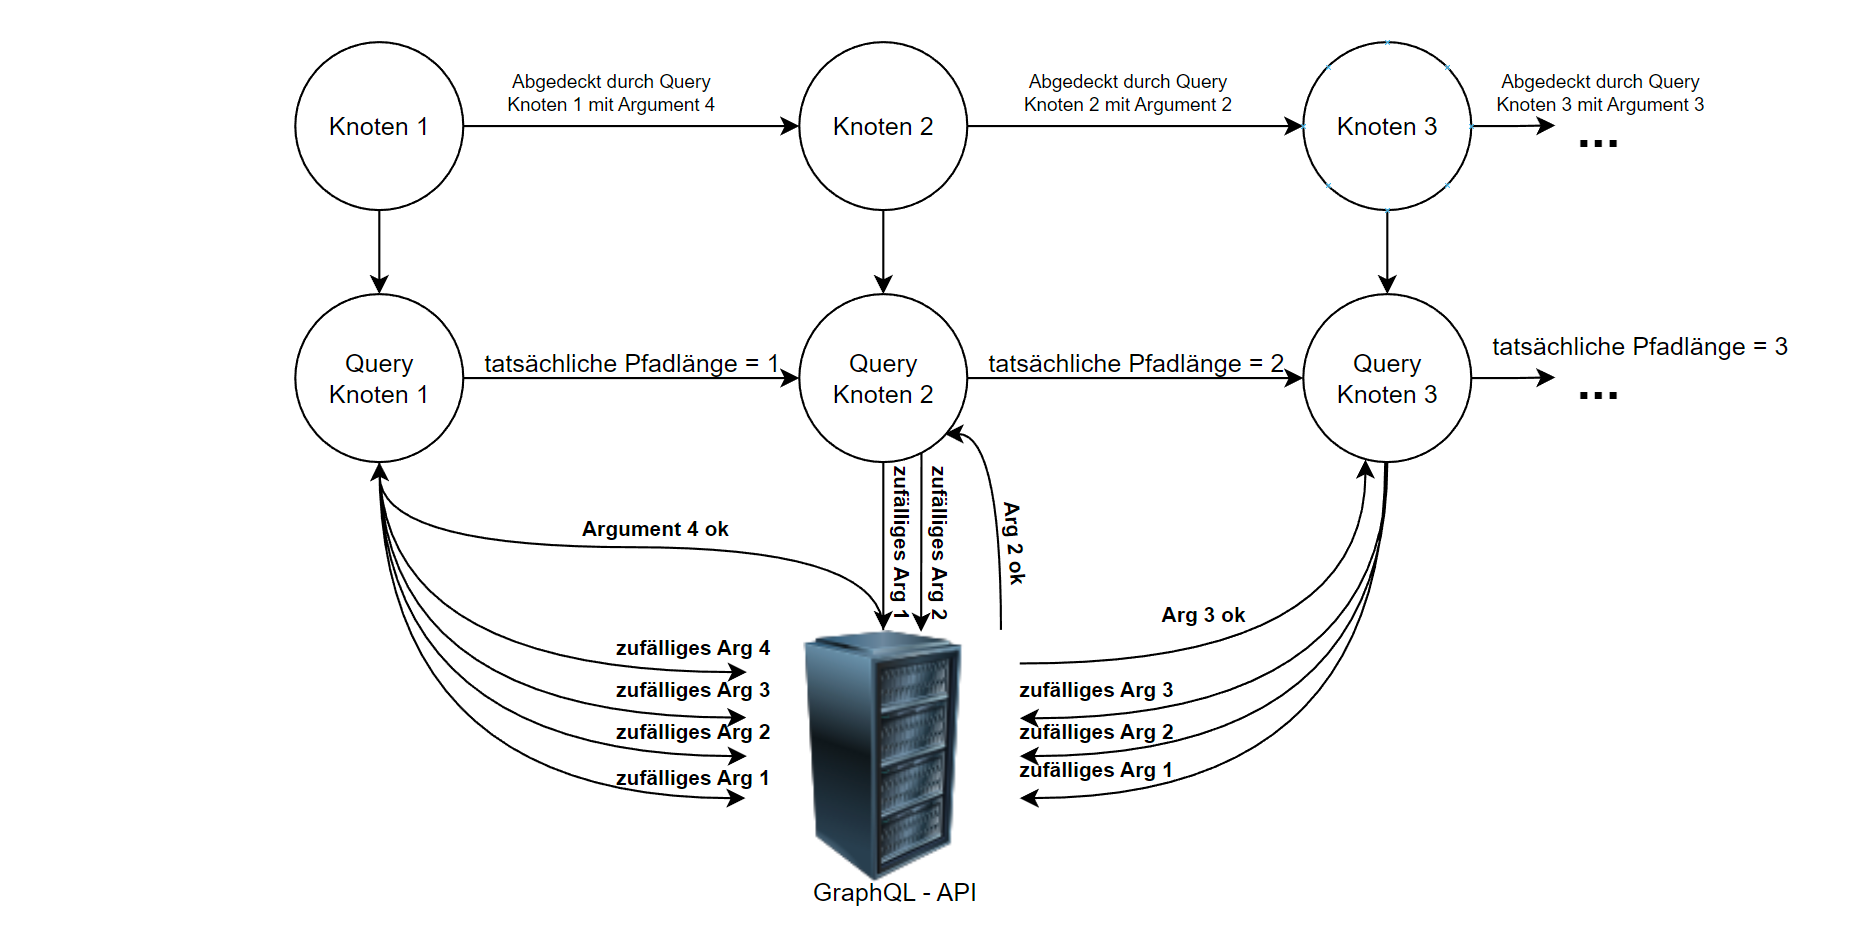
\includegraphics[width=\textwidth,keepaspectratio]{img/ablauffuturework}
    \end{center}
    \caption{Beispielablauf einer adaptiven Generierung}
    \label{adaptive}
\end{figure}

Mögliche Limitierungen wären hierbei jedoch, dass ein Pfad niemals seine gewünschte Pfadlänge erreicht, weil zum Beispiel Daten für den Pfad fehlen und somit jedes Argument unzureichend ist.
Denkbar wäre auch, dass Argumentgeneratoren nicht in der Lage sind, passende Daten zu erzeugen.
Es wären Strategien zu entwickeln, die sicherstellen, dass solche Limitierungen korrekt behandelt werden.
Mit einer solchen Query-Generierung ist eine Steigerung der tatsächlichen Pfadabdeckung möglich und gleichzeitig kann das erlangte Wissen in anderen Pfaden genutzt werden, um die Argumentgenerierung zu vereinfachen.




